\documentclass[twocolumn,preprintnumbers,superscriptaddress]{revtex4-2}
\usepackage{amsmath}
\usepackage{amssymb}
\usepackage{graphicx}
\usepackage{hyperref}
\usepackage{physics}
\usepackage{xcolor}
\usepackage{xspace,slashed}
\usepackage{qcircuit}
\usepackage{multirow}
\usepackage[utf8]{inputenc}
\usepackage{subfigure}

\usepackage{array}

\newcommand{\commentCBP}[1]{{\color{red} {[C: #1]}}}
 \newcommand{\commentJB}[1]{{\color{blue} {[J: #1]}}}
 \newcommand{\commentMC}[1]{{\color{magenta} {[M: #1]}}}
 \newcommand{\commentAF}[1]{{\color{cyan} {[A: #1]}}}
 \newcommand{\commentDMG}[1]{{\color{orange} {[D: #1]}}}
 \newcommand{\commentSC}[1]{{\color{purple} {[S: #1]}}}

\begin{document}

\title{
  Style-based quantum generative adversarial networks for Monte Carlo events
}

\preprint{CERN-TH-2021-139, TIF-UNIMI-2021-14}

\newcommand{\CERNaff}{Theoretical Physics Department, CERN, CH-1211
  Geneva 23, Switzerland.}

\newcommand{\tii}{Quantum Research Centre, Technology Innovation Institute, Abu Dhabi, UAE}

\newcommand{\bern}{Albert Einstein Center, CH-3012 Bern, Switzerland}

\newcommand{\UB}{Departament de F\'isica Qu\`antica i Astrof\'isica and Institut de Ci\`encies del Cosmos (ICCUB), Universitat de Barcelona, Barcelona, Spain.}

\newcommand{\MIaff}{TIF Lab, Dipartimento di Fisica, Universit\`a degli Studi di
  Milano and INFN Sezione di Milano, Milan, Italy.}

\author{Carlos Bravo-Prieto}
\affiliation{\tii}
\affiliation{\UB}

\author{Julien Baglio}
\affiliation{\CERNaff}

\author{Marco C\`e}
\affiliation{\CERNaff}

\author{Anthony Francis}
\affiliation{\bern}

\author{\\Dorota M. Grabowska}
\affiliation{\CERNaff}

\author{Stefano Carrazza}
\affiliation{\MIaff}
\affiliation{\CERNaff}
\affiliation{\tii}


\begin{abstract}
We propose and assess an alternative quantum generator architecture in the context of generative adversarial learning for Monte Carlo event generation, used to simulate particle physics processes at the Large Hadron Collider (LHC). We validate the methodology by implementing the quantum network on artificial data generated from known underlying distributions. The network is then applied to Monte Carlo-generated datasets of specific important LHC scattering processes. The new quantum generator architecture leads to an improvement in state-of-the-art implementations while maintaining shallow depth networks. Moreover, the quantum generator successfully learns the underlying distribution functions even if trained with small training sample sets; this is particularly interesting for data augmentation applications. We deploy this novel methodology on two different quantum hardware architectures, trapped-ion and superconducting technologies, to test its hardware-independent viability.  
\commentCBP{Carlos}
 \commentJB{Julien}
 \commentMC{Marco}
 \commentAF{The label (Revisit) denotes sentences where I'm working on an alternative but think we should clarify or change sth}
 \commentDMG{Dorota}
 \commentSC{Stefano}


\end{abstract}

\maketitle

\section{Introduction}

Quantum computing is a new paradigm whereby quantum phenomena are harnessed to perform computations. The current availability of noisy intermediate-scale quantum (NISQ) computers ~\cite{nisq}, and recent achievements such as quantum computational supremacy~\cite{supremacy, zhong2020quantum}, have led to a growing interest in these devices to perform computational tasks faster than any classical machine. Among many of the near-term applications~\cite{cerezo2021variational, bharti2021noisy}, the field of Quantum Machine Learning (QML)~\cite{biamonte2017quantum, schuld2018supervised} is held as one of the most promising approaches to make use of NISQ computers.

Early work in QML was mostly focused on speeding up linear algebra subroutines~\cite{wiebe2012quantum, lloyd:2013ml, Rebentrost:2014svm, kerenidis2020quantum}, widely used in classical machine learning, by leveraging the Harrow-Hassidim-Lloyd
algorithm~\cite{harrow2009quantum}. This approach is promising, though its utility depends on the existence of large-scale quantum computers with low gate errors and enough qubits to perform quantum error correction. More recent proposals focus on defining a quantum neural network (QNN), or parameterized quantum circuit~\cite{benedetti2019parameterized, sim2019expressibility, bravo2020scaling, larocca2021theory}, which then can be trained to implement a function class~\cite{schuld2021effect, goto2021universal, perez2021one}; these proposals can be implemented on current NISQ-era devices. For example, several QNNs have been proposed for pattern classification~\cite{havlivcek2019supervised, Schuld:2020circuit, perezsalinas:2020reuploading, dutta2021realization} or data compression~\cite{romero2017quantum, pepper2019experimental, bravo2021quantum, cao2021noise}. This QML approach to quantum computing is a research topic that can be adapted, improved, and tested on many research problems in disparate scientific fields. Motivated by this idea, we propose to investigate the possibility of using QNNs for generative modeling~\cite{benedetti2019generative, hamilton2019generative, coyle2020born}. More specifically, we explore the uses of QNNs for the generation of Monte Carlo events through quantum generative adversarial networks (qGANs)~\cite{dallaire2018quantum, lloyd2018quantum}.

The generative adversarial framework employs two competing networks, the generator and the discriminator, that are
trained alternatively~\cite{goodfellow2014generative}. The generator produces candidates
while the discriminator evaluates them. The objective of the discriminator is to
distinguish the real samples from the generated ones. That is, the discriminator
plays the role of the generator's adversary, and therefore, their competition is
a zero-sum two-player game. By substituting either the discriminator, the
generator, or both with quantum systems, we translate the scheme to quantum
computing.

In recent months, the spreading interest in QML has led to different qGAN
implementations~\cite{zoufal2019quantum, zeng2019learning, situ2020quantum, hu2019quantum, benedetti2019adversarial, romero2021variational, niu2021entangling}. Our contribution here can be summarized in three distinct aspects. (1) Previous proposals employed toy data for their qGAN training. In contrast, we test our model using data for a quantum scattering process. In particular, we first train and validate our qGAN model with artificial data from known underlying probability density functions. Then, in order to test our model in a realistic set-up, we use as training sets simulated Monte Carlo events for particle physics processes at the Large Hadron Collider (LHC) at CERN. (2) We propose an alternative quantum generator architecture. Traditionally, the prior noise distribution, or latent dimension in the language of generative models, is provided to the quantum generator through its first quantum gates. We instead embed it on every layer of the network. This allows us to achieve improved state-of-the-art results with shallow QNNs. Note that a similar concept was introduced in the classical context~\cite{karras2019style}, coined as style-based GAN; it was proven to be extremely useful. Given this analogy with the classical literature, from now on we refer to our qGAN model as style-qGAN. (3) We validate and assess our style-qGAN in quantum hardware. Specifically, we successfully implement our model in two different quantum architectures, namely, ion traps and superconducting qubits.

It is important to highlight that several research groups from the high-energy
physics (HEP) community are investigating potential applications of quantum
technologies in HEP applications and obtaining interesting
results~\cite{P_rez_Salinas_2021,Guan_2021,chang2021quantum,Chang_2021,Belis_2021,khattak2021fast}.
Therefore, the study presented in this manuscript should be considered as
proof-of-concept, providing a robust and reproducible starting point for future
investigations. In particular, the introduction of GAN models in HEP Monte Carlo
simulation has been discussed extensively in the last years, see
Refs.~\cite{baldi2021gan,Backes_2021,butter2020generative,Butter_2021,Butter_2020,Bellagente_2020,Butter_2019}.
In this work, we consider the possibility to use a qGAN model in a data
augmentation context, where the model is trained with a small amount of input
samples and it learns how to sample the underlying distribution.

% To be modified
The paper is structured as follows. In Sec.~\ref{sec:implementation} we define our style-qGAN model. In Sec.~\ref{sec:validation} we
validate the style-qGAN model using toy data. Then, in Sec.~\ref{sec:lhc} we train the style-qGAN
generator on simulated LHC events. Finally, in Sec.~\ref{sec:deployment} we test
our final model on real quantum hardware, and in Sec.~\ref{sec:conclusion} we
present our conclusion and future development directions. \commentJB{We present in Appendix.~\ref{sec:appendixnoise} a noise simulation
  of the algorithm using the simplified noise model provided by IBM~Q for the target machine we have used with IBM~Q hardware.}

\section{Implementation}
\label{sec:implementation}

\subsection{Workflow design}

The classical implementation of a GAN model~\cite{goodfellow2014generative}
involves at least three required components: the discriminator model, the
generator model, and the adversarial training procedure. In this work we
consider a hybrid quantum-classical system, where the generator model has a
quantum representation through a QNN while the
discriminator is a classical neural network model. This choice is motivated by
the practical positive implications of a hardware-based generative model, in
particular the possibility to obtain performance improvements in a real quantum
device. The idea of using a quantum device for the generation of
samples is very attractive because the complicated aspects of density modelling and sampling are delegated to a hardware architecture.

%
There are alternative approaches where both models could be represented by a
QNN~\cite{dallaire2018quantum, hu2019quantum, benedetti2019adversarial, romero2021variational, niu2021entangling}. However, after testing some prototype architectures, we have observed faster convergence when using a classical discriminator.

In Figure~\ref{fig:scheme} we schematically show the steps involved in the style-qGAN
presented here. The procedure starts from the preparation of reference samples from a
known distribution function that we would like to encode in the quantum
generator model. At the same time, we define a QNN model where
we inject stochastic noise in the latent space variables; these are used to
define all the quantum gates of the network. The generator model is then used to extract fake generated samples
that, after the training procedure, should match the quality of the known input
distribution. Lastly, both sets of samples are used to train the discriminator
model. The quality of the training is measured by an appropriate loss function
which is monitored and optimized classically by a minimization algorithm based on
the adversarial approach. The training process consists of simultaneous
stochastic gradient descent for both models which, after reaching convergence,
delivers a quantum generator model with realistic sampling.

In the next paragraphs, we first introduce the optimization procedure and the quantum
generator network, and validate the procedure by using reference samples from known
distribution functions and quantum simulation on classical hardware. We then
train our style-qGAN model with Monte Carlo-generated LHC events using quantum
simulation. Finally, the best-trained model is deployed on real quantum hardware
devices based on superconducting and trapped-ion technologies.

All calculations involving quantum circuit simulation are performed using
{\tt Qibo} v0.1.6~\cite{efthymiou2020qibo,stavros_efthymiou_2021_5088103} on
classical hardware. For this particular project, we have used the {\tt
tensorflow}~\cite{tensorflow2015-whitepaper} backend which provides the
possibility to use gradient descent optimizers during the training step. The
style-qGAN model is publicly available through the {\tt Qibo}
documentation~\cite{add_cite_tutorial}. Furthermore we extended the model implementation to run on quantum hardware by embedding {\tt OpenQASM}~\cite{cross2017open} code generated by {\tt Qibo} into a {\tt Qiskit}~\cite{gadi_aleksandrowicz_2019_2562111} based framework. This code is also openly available~\cite{add_cite_tutorial}. \commentJB{We have also translated the algorithm to Amazon \texttt{Braket SDK} in order to run our code on ionQ machines accessible via Amazon Web Services.}


\begin{figure}
  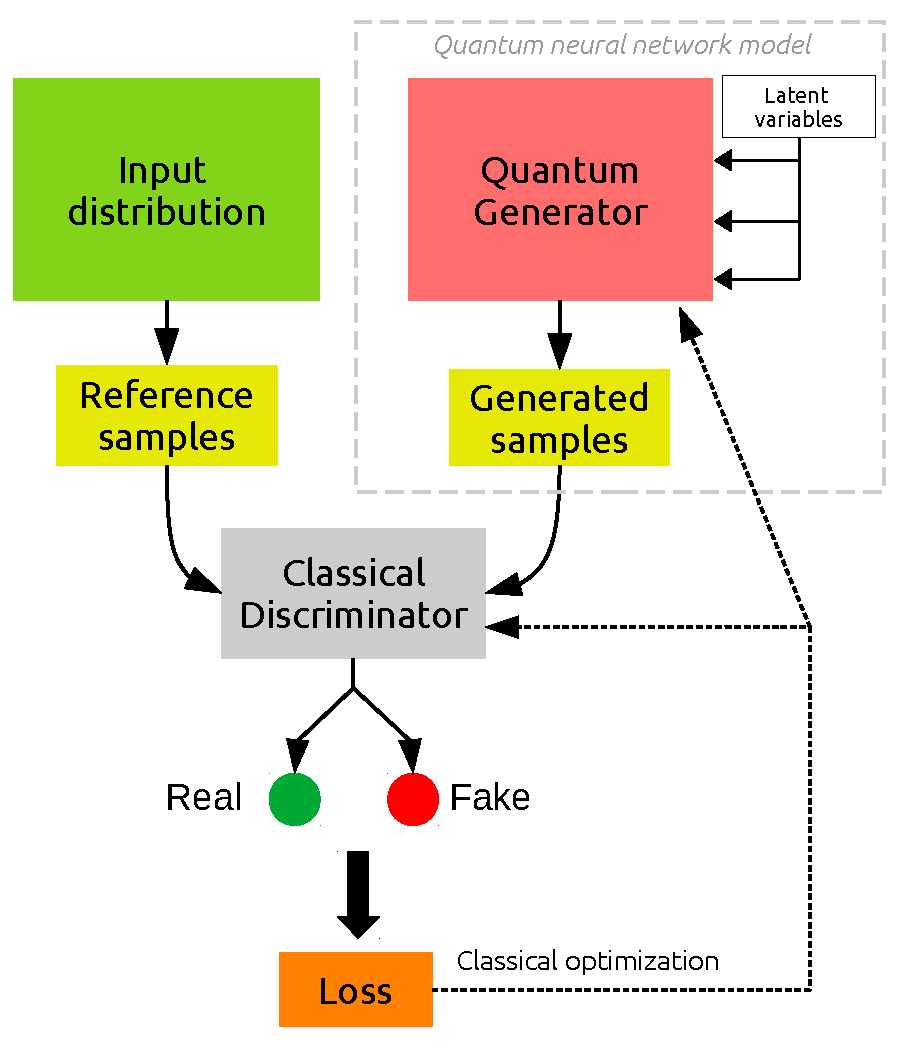
\includegraphics[width=0.4\textwidth]{plots/scheme2.pdf}
  \caption{\label{fig:scheme} Schematic steps involved in the style-qGAN training.}
\end{figure}

\subsection{Optimization procedure}

As previously discussed, our style-qGAN comprises of a QNN for the generator $G(\phi_g)$ and a classical network for the discriminator $D(\phi_d)$. The quantum generator transforms samples from a prior standard Gaussian noise distribution $z \sim p_{prior}(z)$, also called latent variables, into samples generated by $G(\phi_g)$, thus mapping $p_{prior}(z)$ to a different distribution $p_{fake}$ of generated data. On the other hand, the discriminator takes as input samples $x$ and tries to distinguish between fake data from the generator and real data from the reference input distribution $p_{real}$. The training corresponds to an adversarial game, where we alternate between improving the discriminator to distinguish fake and real data, and the generator to cheat the discriminator with new fake data.

In this work, we consider the binary cross-entropy for the optimization objective. The generator's loss function can be defined as
\begin{equation}
  \mathcal{L}_G(\phi_g,\phi_d) = -\mathbb{E}_{z \sim p_{prior}(z)}[\log D(\phi_d,G(\phi_g,z))]  \,,
\end{equation}
while the discriminator's loss function can be defined as
\begin{equation}
\begin{split}
  \mathcal{L}_D(\phi_g,\phi_d) = \mathbb{E}_{x \sim p_{real}(x)}[\log D(\phi_d,x)] \\+\, \mathbb{E}_{z \sim p_{prior}(z)}[\log (1-D(\phi_d,G(\phi_g,z)))]\,.
\end{split}
\end{equation}
Notice that the adversarial training corresponds to a minimax two-player game,
\begin{equation}
 \underset{\phi_g}{\min}\,\,\mathcal{L}_G(\phi_g,\phi_d)  \,,
\end{equation}
\begin{equation}
 \underset{\phi_d}{\max}\,\,\mathcal{L}_D(\phi_g,\phi_d)  \,,
\end{equation}
where the optimum uniquely corresponds to the Nash equilibrium between the loss functions.

The optimization of the parameters $\phi_g$ and $\phi_d$ is done alternatively by updating the quantum generator and classical discriminator. The optimizer used to update the steps in this work is the ADADELTA~\cite{zeiler2012adadelta}, which is a stochastic gradient descent method that monotonically decreases its learning rate. To be precise, the starting learning rates utilized are $0.1$ for the classical discriminator and $0.5$ for the quantum generator.

\subsection{Quantum generator architecture}
The quantum generator is implemented by a QNN with trainable parameters. In particular, we employ the architecture shown in Figure~\ref{fig:circuit}. We consider a layered QNN, where each layer is composed of a set of entangling gates $U_{\rm ent}$ preceded by two alternating $R_y$ and $R_z$ single-qubit rotations. After implementing the layered network, a final layer of $R_y$ gates is applied. Note that $U_{\rm ent}$ is specific to each example and $R_j(\theta_k) = e^{-i\theta_k \sigma_j /2}$. \commentAF{(Revisit) could add some more info: why 2 alternating rotations, number of parameters per layer excluding entangling gates, highlight that the gate count depends on the problem}
Additionally, the number of layers can be modified to tune the capacity of the quantum generator. However, in the following we obtain state-of-the-art results with shallow QNNs with only one and two layers.
\commentAF{changed "However, as we shall see in the following sections, we manage to obtain improved state-of-the-art results with shallow QNNs, namely, with only one and two layers."} \commentCBP{I think it is important to specify that our results \textit{improve} the state-of-the-arts results for qGANs. Obviously we do not improve with respect classical techniques.}
\commentAF{Good point. If we want to write this we need to explain how and in what way we improve. We could add this in the following sections explicitly mentioning the improvements other qGANs. Alternatively we could add a sentence here, but then it might be better situated at the end of section I. } \commentCBP{Let me put here the points we improve. (1) Higher binning density (at least 1 order of magnitude higher) (2) Even with the higher binning density we obtained smaller KL divergences (3) We use a real setup (non-toy data)}

Let us emphasize here the novelty of the quantum generator architecture used for the style-qGAN model, where the action of each qubit rotation is parameterized by the set of trainable parameters $\phi_g$ and, most importantly, the latent vector $\xi$. Specifically, we encode them by using a linear function as
\begin{equation}
    \label{eq:rotation} R_{y,z}^{(i,j)}\left(\phi_g, \xi\right) = R_{y,z}\left(\phi_g^{(i)} \xi^{(j)} + \phi_g^{(i+1)}\right)\,,
\end{equation}
where $i,j$ indicates the component of the vector. The length of the latent vector $\xi$ will depend on the choice of latent dimension $D_{latent}$ for each implementation. Notice that our quantum generator embeds the input latent variables into all the quantum gates of the network, in contrast to previous qGAN proposals. This permits the new architecture to process and decide in which
parts of the QNN the latent variables should play a relevant role.

\begin{figure}
  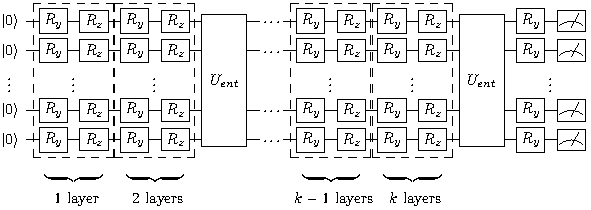
\includegraphics[width=1.0\columnwidth]{plots/ansatz1.pdf}
  \caption{\label{fig:circuit}Quantum neural network employed for the qGAN model. As indicated by the dashed box, each layer is composed of a set of entangling gates $U_{\rm ent}$, to be specified for each example, preceded by two alternating $R_y$ and $R_z$ single-qubit rotations. After implementing the layered network, a final layer of $R_y$ gates is applied.}
\end{figure}

Recall that the quantum generator's task is creating fake samples to fool the classical discriminator. The fake samples are prepared by acting with the parameterized QNN on the initial $n$-qubit state $\ket{0}^{\otimes n}$, and then measuring in the computational basis. For our implementations, each qubit delivers one sample component. That is, the sample $x \in \mathbb{R}^n$ is generated as
\begin{equation}
    \label{eq:samples} x = \left[-\left\langle\sigma_z^1\right\rangle,-\left\langle\sigma_z^2\right\rangle,\hdots,-\left\langle\sigma_z^n\right\rangle\right]\,,
\end{equation}
with
\begin{equation}
    \label{eq:expectation}\left\langle\sigma_z^i\right\rangle = \left\langle\Psi(\phi_g,\xi)\left|\,\sigma_z^i\,\right|\Psi(\phi_g,\xi)\right\rangle \,,
\end{equation}
where $\Psi(\phi_g,\xi)$ is the output state from the quantum generator. Notice, however, that for other models, more sophisticated ways of generating fake samples could be more convenient to implement. For instance, one could generate a sample component by computing expectation values involving several qubits. Finally, let us briefly comment that we used a deep convolutional neural network for the discriminator. More details about the classical discriminator implementation can be found in the code~\cite{cite_code}.

\section{Validation examples}
\label{sec:validation}

In this section we show examples of style-qGAN models obtained for known prior
distribution functions in one and three dimensions. The results presented here
have been obtained after a systematic process of fine-tuning and manual
hyper-optimization of the training and quantum generator model.

\subsection{1D Gamma distribution}
\label{sec:gamma}

In order to test the framework proposed above, we
consider the sampling of a 1D gamma distribution with probability density
function reading
\begin{equation}
  p_\gamma (x, \alpha, \beta) = x^{\alpha-1} \frac{e^{-x/\beta}}{\beta^\alpha \Gamma(\alpha)}\,,
\end{equation}
where $\Gamma$ is the Gamma function. In this example we take $p_\gamma (x, 1,
1)$ as the input distribution and train a style-qGAN with 1 qubit, 1 latent dimension and
1 layer using $10^4$ samples from the input distribution. The total number of trainable parameters is 10. We perform a linear pre-processing of the data to fit the samples within $x \in [-1, 1]$. We undo this transformation after the training.
%
In Figure~\ref{fig:loss} we show the evolution of the loss function for the
generator and discriminator models in terms of the number of epochs. We observe the
typical behavior of GAN training and a convergence region after 15000 epochs.
%
The style-qGAN is trained with batch sizes of 128 samples.

\begin{figure}
  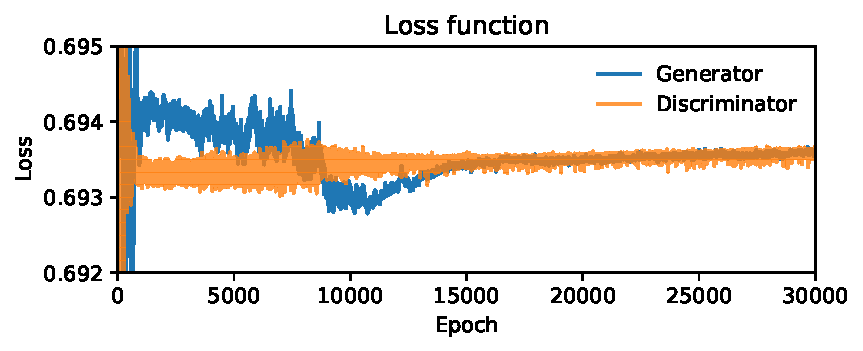
\includegraphics[width=0.5\textwidth]{plots/1Dgamma/1Dgamma_loss.pdf}
  \caption{\label{fig:loss}Example of loss function convergence. After an
  initial warm-up phase, the loss function of both models converges.}
\end{figure}

A necessary property of this framework is that the style-qGAN model can learn the underlying distribution from a small data set. To demonstrate this, we train a style-qGAN model with a set number of reference samples and then use it to generate two sets of samples of different size. In particular we choose to generate sets of $10^4$ and $10^5$ samples.

The top of Figure~\ref{fig:gamma} shows the smaller sample distribution generated by the style-qGAN model in blue and a sampling of the reference distribution of the same size in red. This enables a comparison also using the Kullback-Leibler divergence (KL)~\cite{kullback1951information}.
In both cases the $10^4$ samples have been transformed into histograms with 100 bins linearly spaced on the $x$-axis of the figure. We observe that the distributions are statistically similar even for this high-density binning choice. The KL divergence of two displayed distributions is given in the title of the figure. We find a value of 0.141 which entails a high degree of similarity. 

Going further, in the bottom of Figure~\ref{fig:gamma} we show the same results as in the top on the larger set containing $10^5$ samples. Again, we use for comparison a re-sampling of the reference distribution at the same size as the generated set and show both distributions on a grid with 100 linearly spaced bins. 
%
Having generated an order of magnitude more samples than the training set we observe that the style-qGAN model performs well. Both distributions are visually very close to each other and the KL divergence of 0.041 signals a high degree of similarity. \commentAF{Would like to quantify that it also agrees better than before}

%
This behavior confirms that the style-qGAN model is able to learn the underlying
distribution function even if trained with a small training sample set. Such a
feature is particularly interesting in the context of data augmentation
applications~\cite{frid2018synthetic,tanaka2019data}, where few samples are
available, nonetheless the style-qGAN model can generalize and learn the underlying distribution
with satisfactory outcome.


\begin{figure}
  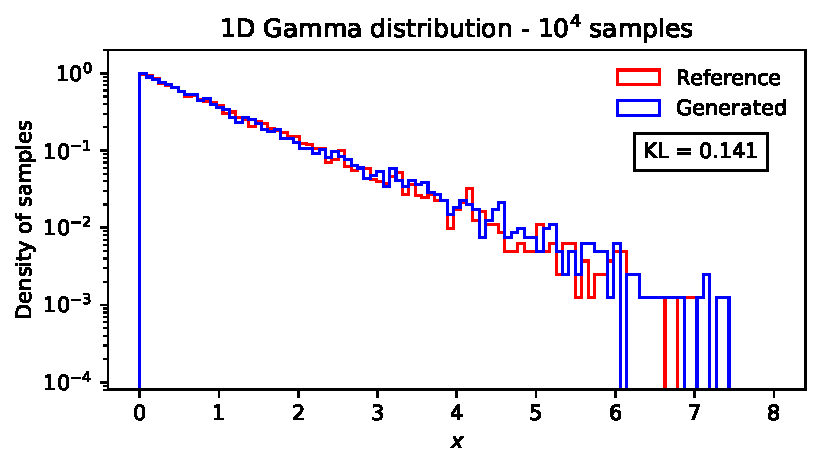
\includegraphics[width=0.45\textwidth]{plots/1Dgamma/1Dgamma_distribution_10k.pdf}
  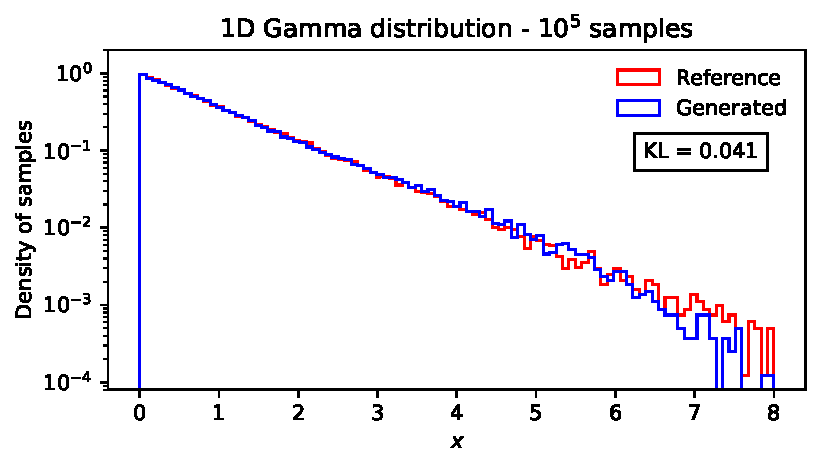
\includegraphics[width=0.45\textwidth]{plots/1Dgamma/1Dgamma_distribution_100k.pdf}
  \caption{\label{fig:gamma} Examples of 1D gamma distribution sampling for the
  reference underlying distribution (red) and a style-qGAN model (blue) that has been
  trained with $10^4$ reference samples. On the top we compare $10^4$ generated samples, while
  on the bottom, $10^5$ generated samples from the same style-qGAN model
  trained with $10^4$ reference samples. We observe a good level of agreement between both
  distributions with low values of the Kullback-Leibler distance.}
\end{figure}

\subsection{3D correlated Gaussian distribution}

The previous test shows that a style-qGAN model implemented on a single qubit can be
trained and produce acceptable results. However, this particular set-up does not
include entanglement between qubits. In order to study the impact of the
entanglement term $U_{\rm ent}$ in the considered QNN, we select as an
underlying distribution a 3D correlated Gaussian distribution centered at
$\overline{\mu}=(0,0,0)$ with covariance matrix
\begin{equation}
\label{eq:covmat}
  \sigma =
\begin{pmatrix}
  0.5 & 0.1 & 0.25\\
  0.1 & 0.5 & 0.1\\
  0.25 & 0.1 & 0.5\\
  \end{pmatrix}.
\end{equation}

For this specific set-up, we consider a 3-qubit model with 3 latent dimensions and
1 layer. The $U_{\rm ent}$ consists of two controlled-$R_{y}$ gates acting sequentially on the 3 qubits.
The total number of trainable parameters is 34. As in the previous example, we perform a linear pre-processing of the data to fit the samples within $x \in [-1, 1]$, and then we undo this transformation after the training. In Table~\ref{table:summary}
we summarize the style-qGAN configurations obtained for both examples discussed in
this section.

Following the same training procedure employed in Section~\ref{sec:gamma}, in
the first row of Figure~\ref{fig:3dgauss} we show $10^5$ samples produced by the
style-qGAN model in two-dimensional projections. Also for this example we use a
grid of 100 linearly spaced bins per dimension in order to highlight small
differences between the prior reference distribution and the artificial samples.
%
In the second row of Figure~\ref{fig:3dgauss} we compare the one dimensional
cumulative projections of samples generated by the style-qGAN model with the
reference input distribution function (red histogram) for $10^5$ samples. Also
for this example, we observe that the distributions are statistically similar,
in fact, the corresponding KL distances are quite small and close to each other.

To further study the features of the style-qGAN model in the third row of plots in Figure~\ref{fig:3dgauss} we show the two-dimensional projections of the ratio between samples generated from the prior reference distribution and the style-qGAN model.
In this way we can visualise how well the model learns not only the distributions but also the correlations between the dimensions of the problem. A ratio of 1, given by a white coloring of the corresponding bin in the figure, would imply the reference and generated samples are identical. Note, since our aim is to generate unseen samples it is not our goal to create a an identical copy of the reference set. At the same time the model should not diverge significantly, depicted by deep blue and red in the figure, or occupy space in the grey area of the figure. 

We observe a good level of agreement, in particular in those regions where the
sampling frequency is larger. The largest deviations are seen at the edges of the distributions, this is on the one hand an artefact from the visualisation due to data augmentation and on the other also a common limitation to the GAN method.

To quantify how well the correlations have been learned beyond 
this level we study the covariance matrices defined by the reference and the generated samples. The summed eigenvalues of the reference and generated covariance matrices give a means to estimate the similarity between the learned underlying correlations. We find agreement between the reference and generated eigenvalues to the better of $\lesssim 10\%$ for style-qGAN set-ups with equal and more than 3 latent dimensions. Recall that the latent variables are introduced in every gate of the circuit, including the entangling ones $U_{ent}$.  With $D_{latent}< 3$ we observe significant deviations of factors $\mathcal{O}(10)$ while for $D_{latent}\geq 3$ no further significant improvement is seen. The same holds for increasing the number of layers in the style-qGAN model. This suggests that the number of latent dimensions introduced are key hyperparameters once the number of layers allows a sufficient complexity.

Since the eigenvalues are known also exactly through Eq.~\ref{eq:covmat} we furthermore can compare the performance of the style-qGAN with increased generation sample size. We find that the style-qGAN with 3 latent dimensions and 1 layer (shown here)
generates sets that reproduce the exact eigenvalues of the input covariance matrix to better than $\lesssim 6\%$ for $10^3$, $\lesssim 1.3\%$ for $5\times10^3$ and $\lesssim 0.8\%$ for $2\times10^4$ samples.

That the larger set of generated samples more closely agrees with the reference input distribution function demonstrated in this way is a key property of a functioning GAN model. The observation that our style-qGAN fulfils this property confirms its viability as functioning quantum implementation of the generative adversarial network idea for multi-dimensional, correlated data.

\commentAF{changed, would like to change order of rows in figure and also text "
The second row of plots in Figure~\ref{fig:3dgauss} shows the ratio between
samples generated from the prior reference distribution and the style-qGAN model. We
observe a good level of agreement, in particular in those regions where the
sampling frequency is larger. We observe that the style-qGAN learns the correlations
between the three dimensions.

In the last row of Figure~\ref{fig:3dgauss} we compare the one dimensional
cumulative projections of samples generated by the style-qGAN model with the
reference input distribution function (red histogram) for $10^5$ samples. Also
for this example, we observe that the distributions are statistically similar,
in fact, the corresponding KL distances are quite small and close to each other."}

\begin{figure*}
  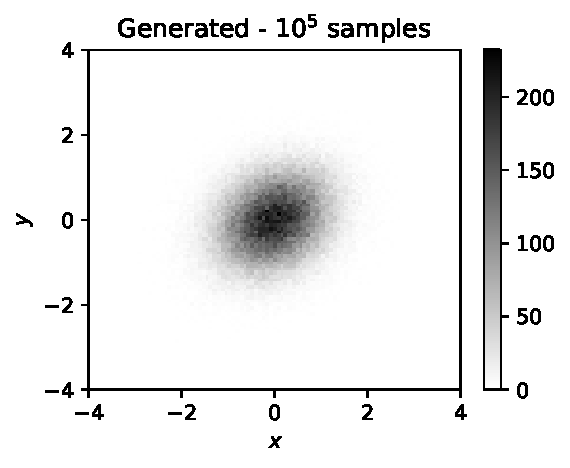
\includegraphics[width=0.3\textwidth]{plots/3Dgaussian_posdef/1-2_FAKE_100k.pdf}%
  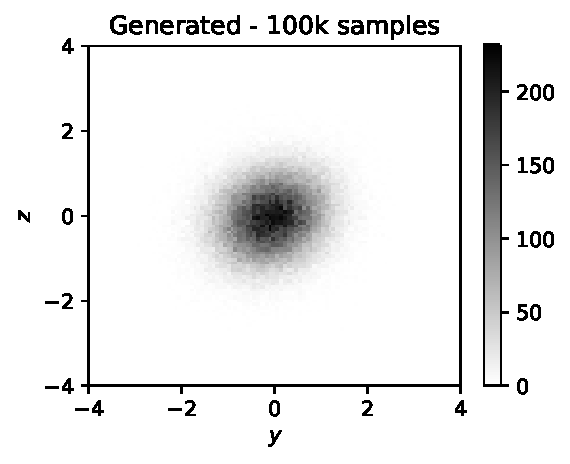
\includegraphics[width=0.3\textwidth]{plots/3Dgaussian_posdef/2-3_FAKE_100k.pdf}%
  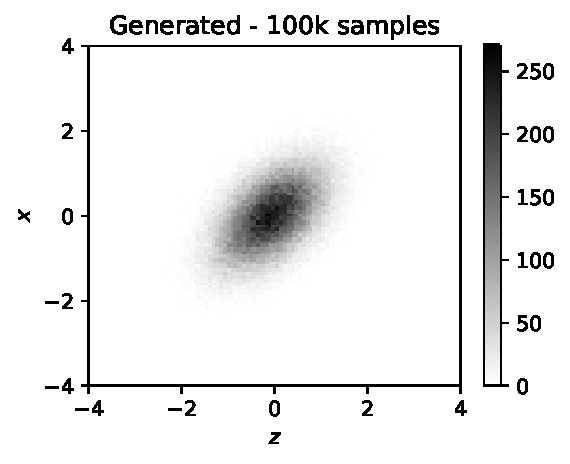
\includegraphics[width=0.3\textwidth]{plots/3Dgaussian_posdef/3-1_FAKE_100k.pdf}

  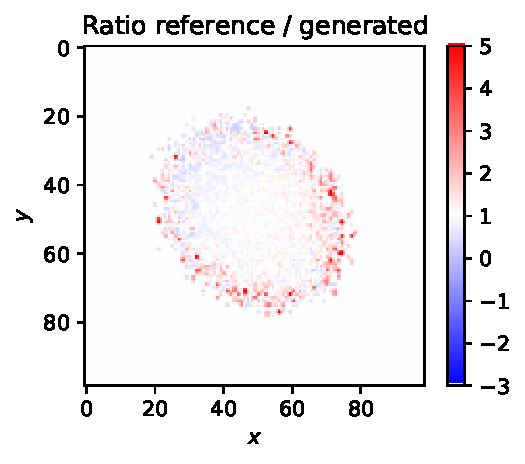
\includegraphics[width=0.3\textwidth]{plots/3Dgaussian_posdef/1-2_RATIO_100k.pdf}%
  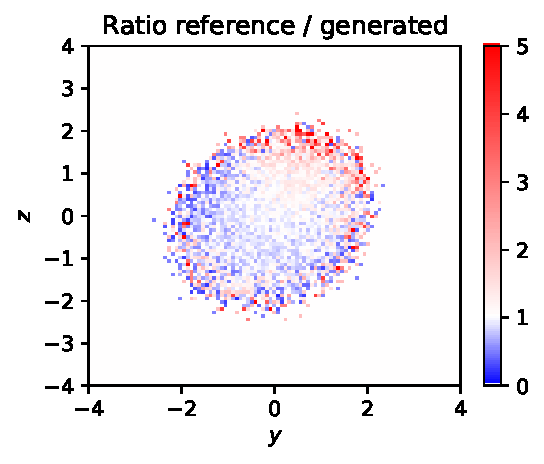
\includegraphics[width=0.3\textwidth]{plots/3Dgaussian_posdef/2-3_RATIO_100k.pdf}%
  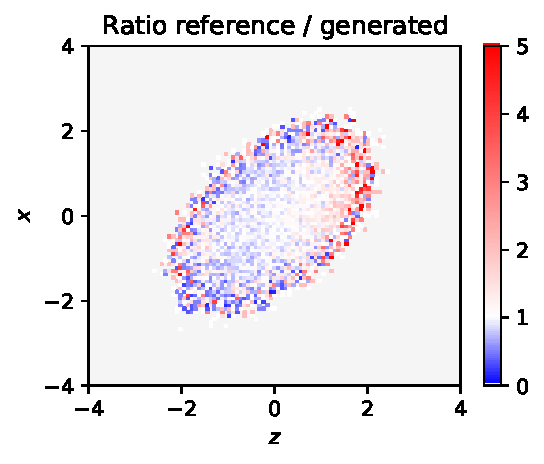
\includegraphics[width=0.3\textwidth]{plots/3Dgaussian_posdef/3-1_RATIO_100k.pdf}

  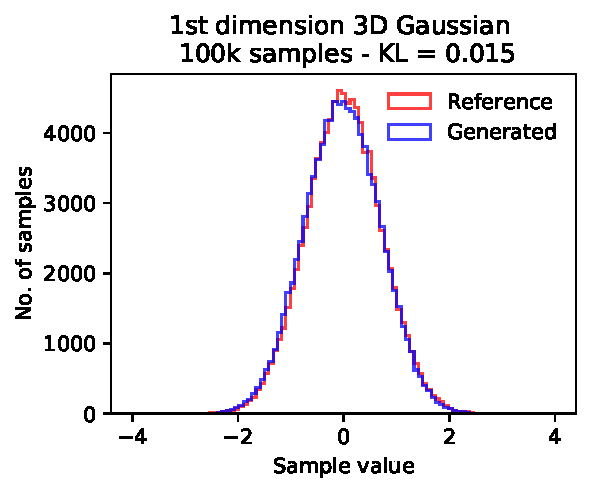
\includegraphics[width=0.29\textwidth]{plots/3Dgaussian_posdef/1-distribution_3dgaussian_100k.pdf}%
  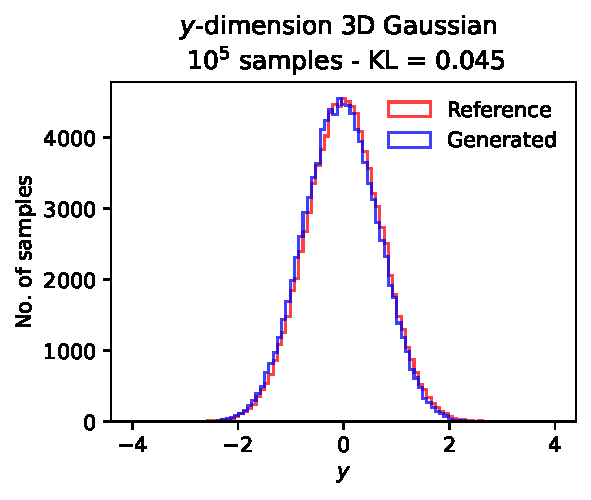
\includegraphics[width=0.29\textwidth]{plots/3Dgaussian_posdef/2-distribution_3dgaussian_100k.pdf}%
  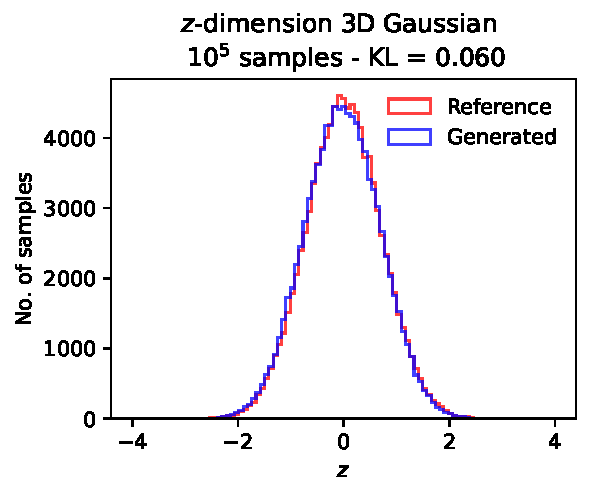
\includegraphics[width=0.29\textwidth]{plots/3Dgaussian_posdef/3-distribution_3dgaussian_100k.pdf}

  \caption{\label{fig:3dgauss}Two-dimensional sampling projections of a 3D
  correlated Gaussian distribution for the style-qGAN model (first row) trained
  with $10^4$ samples and the corresponding ratio to the reference underlying
  prior distribution (middle row). Marginal samples distribution (bottom row)
  for each dimension. The style-qGAN generator model learns the correlations and
  provides acceptable samples when compared to the reference distribution. \commentAF{would like to change row order: $1,2,3 \rightarrow 1,3,2$}}
\end{figure*}

\begin{table}
  \begin{tabular}{l|c|c}
     & {\bf 1D gamma} & {\bf 3D Gaussian} \tabularnewline
    \hline
    Qubits & 1 & 3 \tabularnewline
    $D_{latent}$ & 1 & 3 \tabularnewline
    Layers & 1 & 1 \tabularnewline
    Epochs & $3\times10^4$ & $1.3\times10^4$ \tabularnewline
    Training set & $10^4$ & $10^4$ \tabularnewline
    Batch size & 128 & 128 \tabularnewline
    Parameters & 10 & 34 \tabularnewline
    $U_{\rm ent}$ & None & 2 sequential C$R_y$ gates \tabularnewline
    \hline
  \end{tabular}

  \caption{\label{table:summary} Summary of the style-qGAN set-up for the 1D
  gamma distribution and the 3D correlated Gaussian distribution.}
\end{table}


\section{Generating LHC events}
\label{sec:lhc}

After the validation of the style-qGAN model presented in the previous section
let us consider a training dataset from HEP. One of the big challenges involving
Monte Carlo (MC) event generation is the large number of statistics required to
reconstruct events with high accuracy in order to compare predictions of
physical observables to experimental data. Ideally, we could try
to learn how a specific physical process generates events.

In this context, we have generated $10^5$ MC events for $pp\rightarrow t\bar{t}$
production at LHC with $\sqrt{s} = 13$ TeV with {\tt
MG5\_aMC}~\cite{Alwall:2014hca,Frederix:2018nkq} at leading order in the strong coupling constant. From this simulated events we
sample the Mandelstam variables $(s,t)$ and the rapidity. Here, $s$
and $t$ are understood as the local partonic variables,
$s=(p_1^{}+p_2^{})^2$, $t=(p_1^{}-p_3^{})_{}^2$, where $p_1^{}$ and
$p_2^{}$ are the four-momenta of the incoming quarks within the proton that collide to produce a top quark with four-momentum $p_3^{}$ and an anti-top quark with four-momentum $p_4^{}$, all momenta given in, e.g. the center-of-mass frame.

We consider a 3-qubit model with 5 latent dimensions and 2 layers. Again,
$U_{\rm ent}$ consists of two controlled-$R_{y}$ gates acting sequentially on
the 3 qubits. The total number of trainable parameters is 62. The style-qGAN
model has been trained on $10^4$ samples. See Table~\ref{table:summary_lhc} for more details. In this case, we perform a linear pre-processing of the data
to fit the samples within $x \in [-1, 1]$ after a power
transform~\cite{yeo2000new}. As previously, we undo this transformation after
the training.

Following the same training procedure employed in the previous section, in the
first row of Figure~\ref{fig:ttbar} we show $10^5$ samples produced by the
style-qGAN model in two-dimensional projections. We use a grid of 100 linearly
spaced bins for $y$ and 100 log-spaced bins for $s$ and $t$.
%
The second row of plots in Figure~\ref{fig:ttbar} shows the ratio between
samples generated from the prior original MC distribution and the style-qGAN
model. Again, even for this non-toy model, we observe a remarkable level of agreement, in particular in those regions
where the sampling frequency is larger. Most importantly, we observe as well that the style-qGAN learns
the correlations between the three dimensions. \commentAF{(Revisit) adapt to be like in previous section, also need to dig up the 100k MadGraph samples and perform the eigenvalue analysis, the 10k one is already available}

In the bottom row of Figure~\ref{fig:ttbar} we compare the one dimensional
cumulative projections of samples generated by the style-qGAN model with the
reference input distribution function (red histogram) for $10^5$ samples. Also
for this example, the distributions are statistically similar, with the
corresponding KL distance being small and close to each other.

\begin{figure*}
  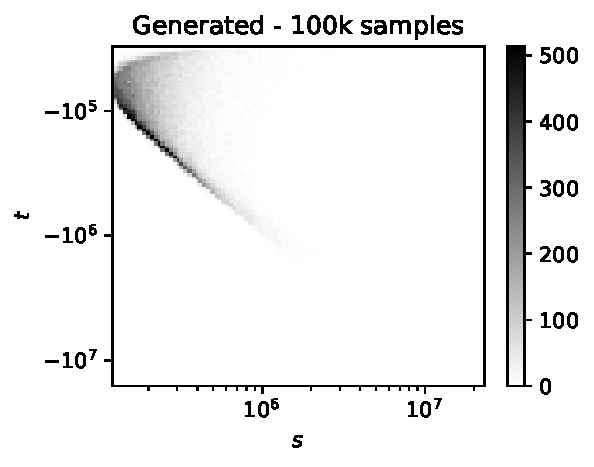
\includegraphics[width=0.32\textwidth]{plots/LHCttbar/s-t_FAKE_100k.pdf}%
  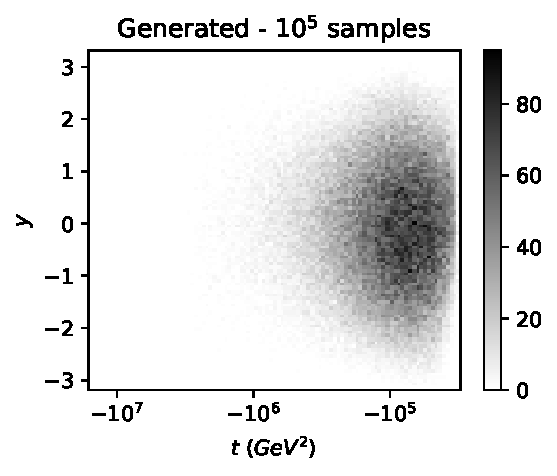
\includegraphics[width=0.3\textwidth]{plots/LHCttbar/t-y_FAKE_100k.pdf}%
  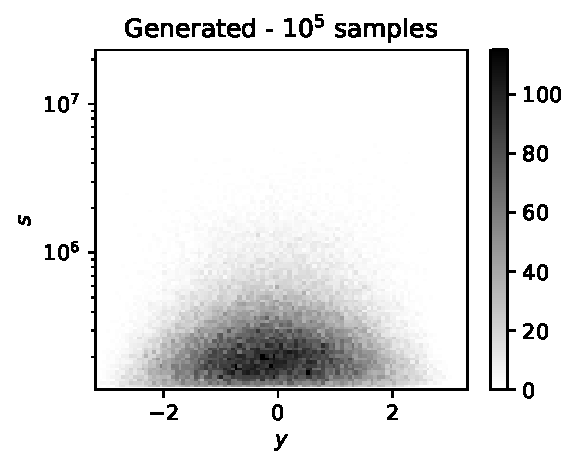
\includegraphics[width=0.31\textwidth]{plots/LHCttbar/y-s_FAKE_100k.pdf}

  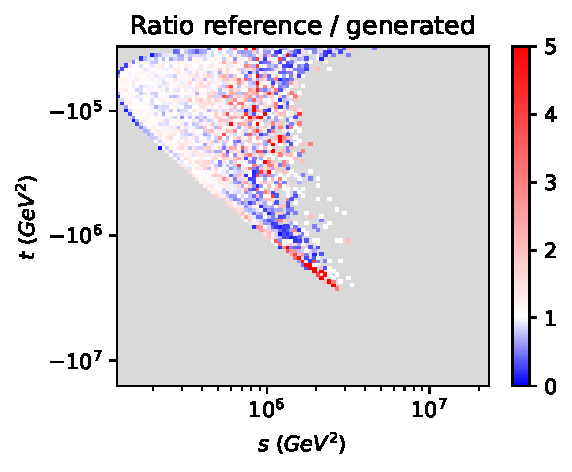
\includegraphics[width=0.32\textwidth]{plots/LHCttbar/s-t_RATIO_100k.pdf}%
  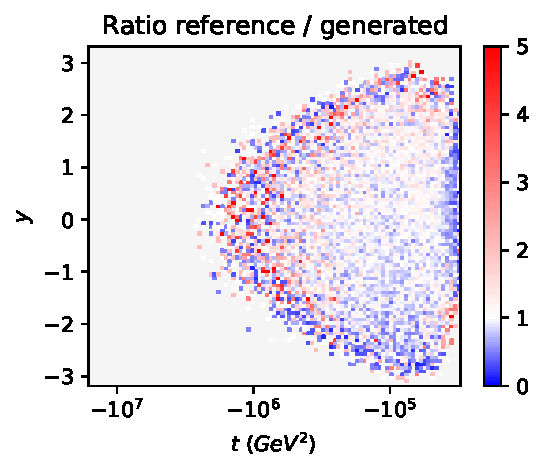
\includegraphics[width=0.3\textwidth]{plots/LHCttbar/t-y_RATIO_100k.pdf}%
  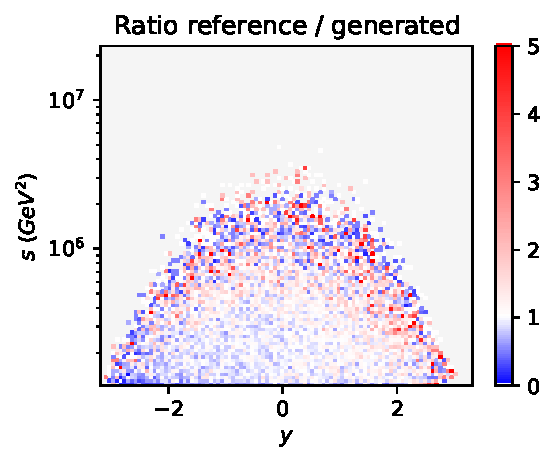
\includegraphics[width=0.31\textwidth]{plots/LHCttbar/y-s_RATIO_100k.pdf}

  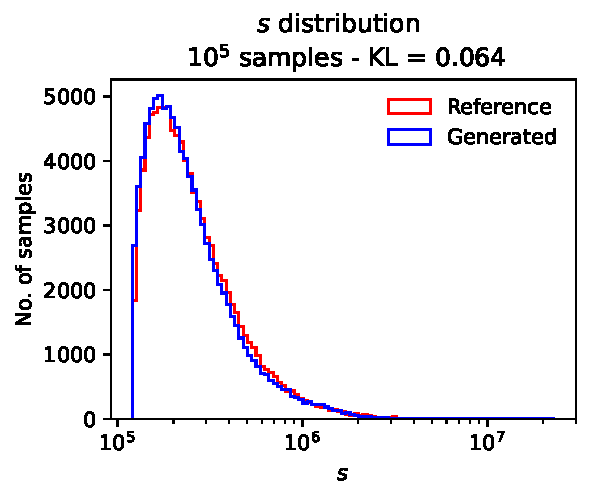
\includegraphics[width=0.29\textwidth]{plots/LHCttbar/s-distribution_LHCdata_100k.pdf}%
  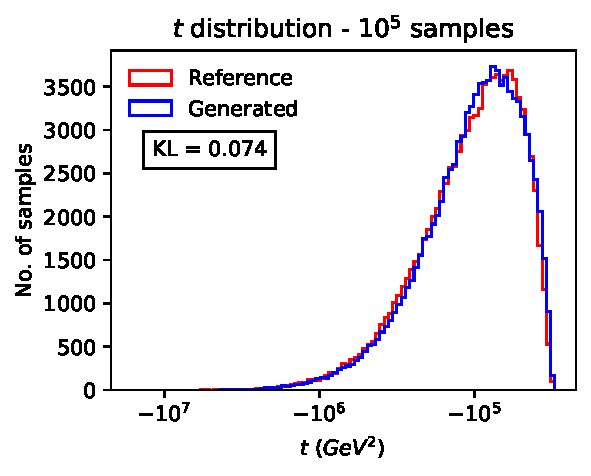
\includegraphics[width=0.29\textwidth]{plots/LHCttbar/t-distribution_LHCdata_100k.pdf}%
  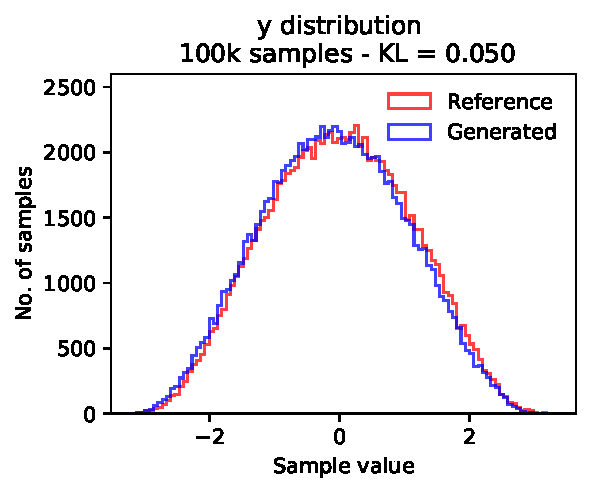
\includegraphics[width=0.29\textwidth]{plots/LHCttbar/y-distribution_LHCdata_100k.pdf}

  \caption{\label{fig:ttbar}Two-dimensional sampling projections for $pp
  \rightarrow t\bar{t}$ production for the style-qGAN model (top row) trained
  with $10^4$ samples and the corresponding ratio to the reference underlying
  prior MC distribution (middle row). Marginal samples distribution (bottom row)
  for each dimension. The style-qGAN generator model learns the correlations and
  provides acceptable samples when compared to the reference distribution.
  \commentAF{would like to change row order: $1,2,3 \rightarrow 1,3,2$}}
\end{figure*}

\begin{table}
  \begin{tabular}{l|c}
     & {\bf $pp \rightarrow t\bar{t}$ LHC events} \tabularnewline
    \hline
    Qubits & 3  \tabularnewline
    $D_{latent}$ & 5 \tabularnewline
    Layers & 2  \tabularnewline
    Epochs & $3\times10^4$ \tabularnewline
    Training set & $10^4$ \tabularnewline
    Batch size & 128 \tabularnewline
    Parameters & 62 \tabularnewline
    $U_{\rm ent}$ & 2 sequential C$R_y$ gates \tabularnewline
    \hline
  \end{tabular}

  \caption{\label{table:summary_lhc} Summary of the style-qGAN set-up for the LHC events distribution.}
\end{table}

\section{Sampling from quantum hardware}
\label{sec:deployment}

In order to benchmark our style-qGAN model on real quantum hardware we
have performed several runs on two different types of
architectures. This allows us to qualitatively assess the impact of
decoherence and noise, issues that are typical for NISQ computers, and
to check whether the model can give already good results without
waiting for error-corrected machines. On the one hand, we have used IBM~Q
quantum computers based on superconducting transmon
qubits~\footnote{\href{https://research.ibm.com/blog/ibm-quantum-roadmap}{IBM's roadmap for scaling quantum technology}, Sept. 2020.}, and, on the other hand, IonQ quantum computers, based on trapped ion technology~\footnote{\href{https://IonQ.com/posts/december-09-2020-scaling-quantum-computer-roadmap}{Scaling IonQ's Quantum Computers: The Roadmap}, Dec. 2020.} and
accessible to us using cloud resources from Amazon Web Services
(AWS).

\commentAF{(Revisit) It could be useful to expand a little more on the implementation here. This is not really featured so far. Possible start:\\
 Going towards real quantum hardware adds a new dimension to our implementation through the number of shots done with each calculation. Furthermore...
 }

\commentJB{
 Going towards real quantum hardware adds a new dimension to our implementation through the number of shots done with each calculation. Indeed, we
 now perform a quantum experiment each time we measure the three-qubit state, and we collect the results after a number of experiment (shots) to build
 up expectation values that are used to create generated samples.

 Prior to send runs on actual quantum hardware, we performed noise simulations using the
IBM~Q simplified noise model provided with the properties of real device backends, to test whether
the results presented in Section~\ref{sec:lhc} would be preserved. Results are provided in Appendix~\ref{sec:appendixnoise}
and show that the impact of the noise is expected to be visible but should not alter too significantly our
results. For the noise simulation as well as the actual runs on IBM~Q quantum devices,}
we have selected in particular the {\tt ibmq\_santiago} 5-qubit Falcon r4L quantum processor.
For our circuit, we need only three qubits with at least one connected to both the other two.
We use a translation layer written in \texttt{Qiskit} between our circuit coded in \texttt{Qibo}
and the quantum hardware to automatically select the three qubits out of the five available
with the best noise properties. Note that this also allows us to test the impact of potential
interference between qubits, as IonQ qubits are fully connected while those of IBM~Q are not.

We present in Figure~\ref{fig:ibm} examples of samples that have been
generated using {\tt ibmq\_santiago} machine on IBM~Q. We use a 3-qubit
model with 5 latent dimensions and 2 layers, which hyperparameters are
the same as the ones used in Section~\ref{sec:lhc} and trained on
$10^4_{}$ samples. To compute each fake sample, we have performed around 1000 shots on the
quantum circuits. We display the generation of $10^5_{}$ samples, as in the previous section,
%of the same amount of samples
in two-dimensional projections. The second row of plots in
Figure~\ref{fig:ibm} shows again the ratio between the reference
samples, generated using the MC event generator, and the samples
generated by the style-qGAN on the {\tt ibmq\_santiago} quantum
hardware. As expected, the agreement is worse than in
Figure~\ref{fig:ttbar} because of the noise, but still quite
reasonable. The
style-qGAN generator model deployed in this NISQ hardware still
manages to capture the correlations and provides reasonably good
samples when compared to the reference distribution.
\commentJB{The KL distances reported in the third row of plots are still relatively small, at most one
  order of magnitude bigger than the KL distances reported in Fig.~\ref{fig:ttbar}.}

\begin{figure*}

  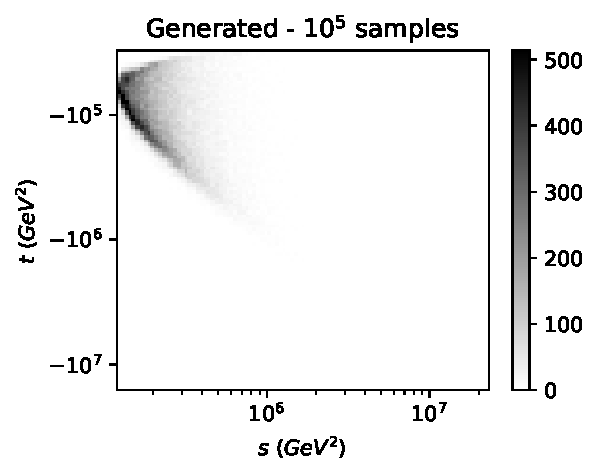
\includegraphics[width=0.32\textwidth]{plots/hardware/ibm_santiago/s-t_FAKE_IBM_100k.pdf}%
  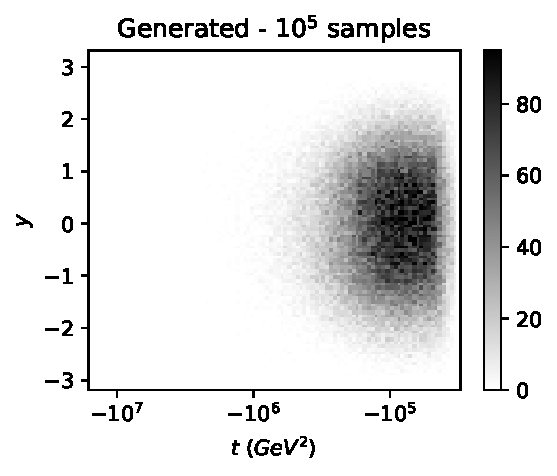
\includegraphics[width=0.305\textwidth]{plots/hardware/ibm_santiago/t-y_FAKE_IBM_100k.pdf}%
  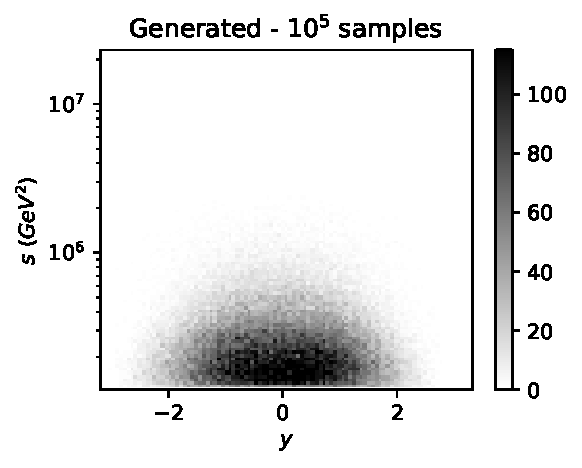
\includegraphics[width=0.31\textwidth]{plots/hardware/ibm_santiago/y-s_FAKE_IBM_100k.pdf}

  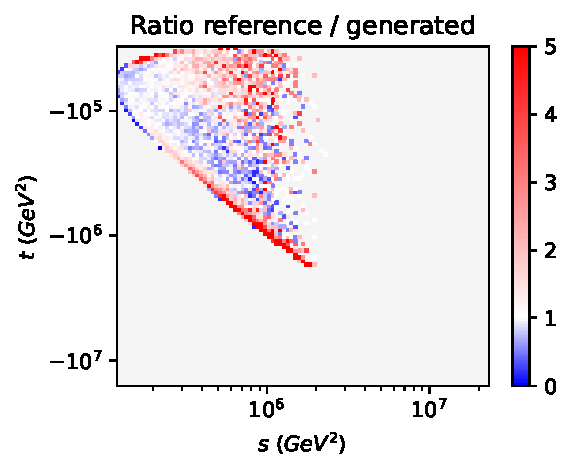
\includegraphics[width=0.32\textwidth]{plots/hardware/ibm_santiago/s-t_RATIO_IBM_100k.pdf}%
  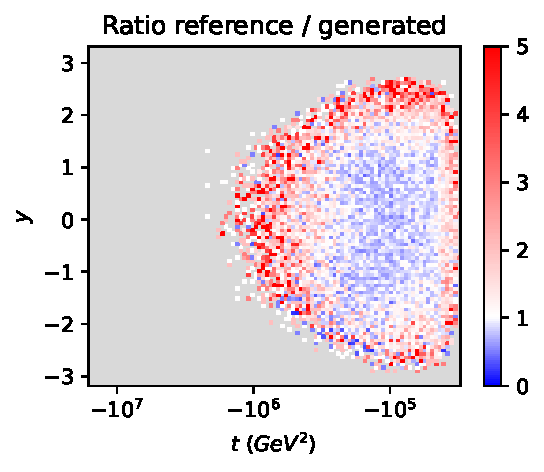
\includegraphics[width=0.305\textwidth]{plots/hardware/ibm_santiago/t-y_RATIO_IBM_100k.pdf}%
  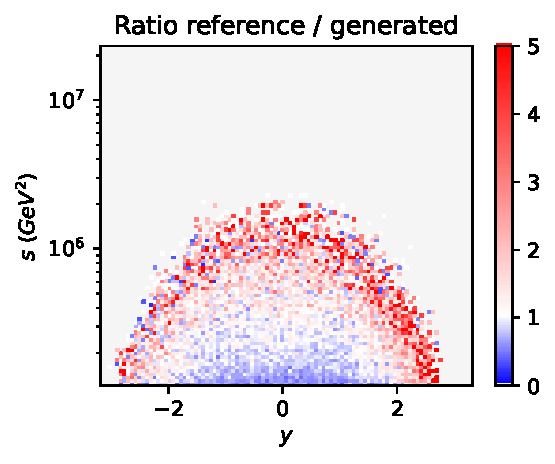
\includegraphics[width=0.31\textwidth]{plots/hardware/ibm_santiago/y-s_RATIO_IBM_100k.pdf}

  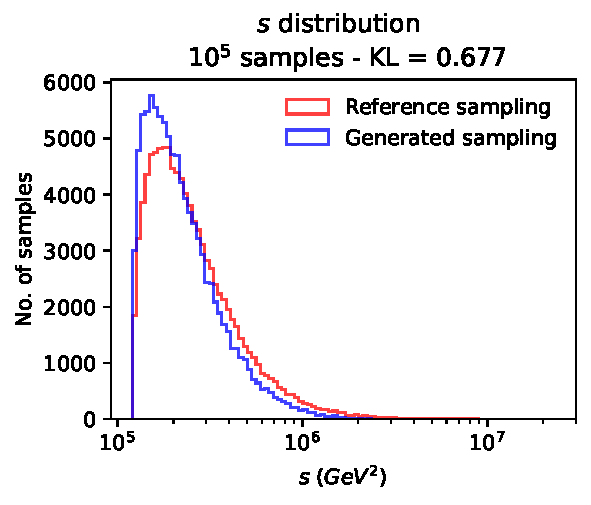
\includegraphics[width=0.29\textwidth]{plots/hardware/ibm_santiago/s-distribution_IBM_LHCdata_100k.pdf}%
  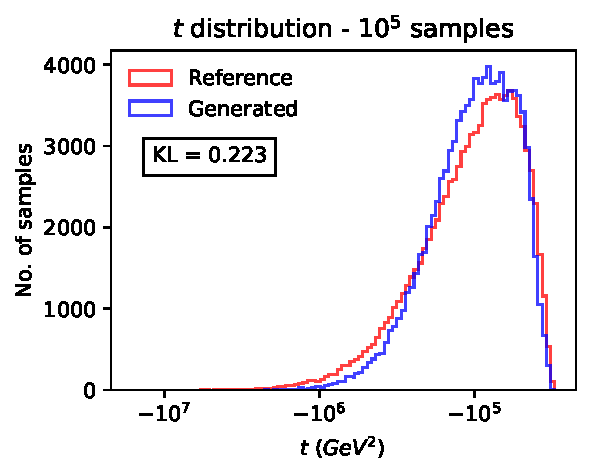
\includegraphics[width=0.29\textwidth]{plots/hardware/ibm_santiago/t-distribution_IBM_LHCdata_100k.pdf}%
  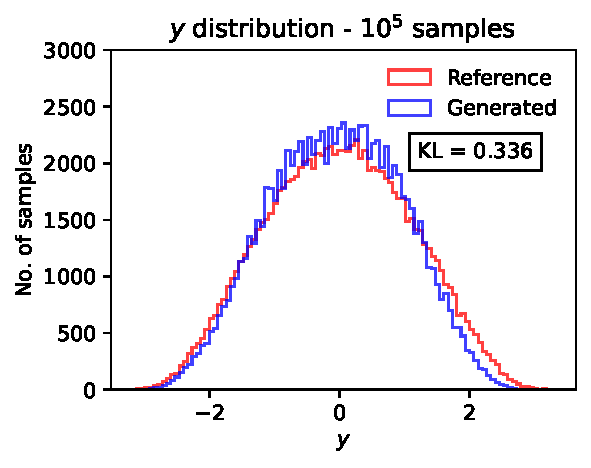
\includegraphics[width=0.29\textwidth]{plots/hardware/ibm_santiago/y-distribution_IBM_LHCdata_100k.pdf}

  \caption{\label{fig:ibm}Example of two-dimensional sampling projections for
  $pp \rightarrow t\bar{t}$ production using the style-qGAN generator
  model on {\tt ibmq\_santiago} (top row) trained with $10^4$ samples and
  the corresponding ratio to the reference underlying prior MC
  distribution (middle row). Marginal samples distribution (bottom row)
  for each dimension. \commentAF{would like to change row order: $1,2,3 \rightarrow 1,3,2$}}
\end{figure*}

\commentAF{ idea:
During the current $NISQ$-era the different quantum hardware architectures pose limits on applications that they can perform. Here, we study how the style-qGAN  performs across different quantum hardware. The aim is to understand whether and to what extent its performance is hardware dependent and its potential hardware transferability. To this extent we performed calculations generating $10^3$ samples each on IonQ machines and seperately on IBM~Q
machines. The fairly small amount of samples available is mainly due to cost constraints.
}


In order to \commentJB{test different} quantum technologies we have also performed a run
with $10^3$ samples only on IonQ machines, compared to a run on IBM~Q
machines with also $10^3$ samples. We have selected this fairly small
amount of samples mainly because of cost constraints to access IonQ on
AWS.
\commentJB{We use again a translation layer, written in Python with the
\texttt{Braket SDK} from Amazon, between our circuit and the quantum hardware, and we
have also performed around 1000 shots for the measurement of the quantum circuit.
Note that the amount of samples is quite low, but the purpose of this test is to assess
how the algorithm performs on different quantum technologies using the same amount of
samples, not to obtain fine-grained results, because of the constraints of our deployment
on IonQ machines.} We show in Figure~\ref{fig:ionq} the two-dimensional projections using
\commentJB{IBM~Q  {\tt ibmq\_santiago} machine (upper row) and IBMQ machine (lower row).
It is clear that the sampling is sparser than in Figure~\ref{fig:ibm}, due to the lower number of
samples, nonetheless it appears that the style-qGAN is already capturing the underlying
distribution and correlations. This is particularly visible on the left plots for the $t-s$ correlation.
The comparison between the upper row and the lower row also indicates that both architectures
obtain similar results. The style-qGAN can give good results on two different quantum harware
technologies.}

\begin{figure*}
  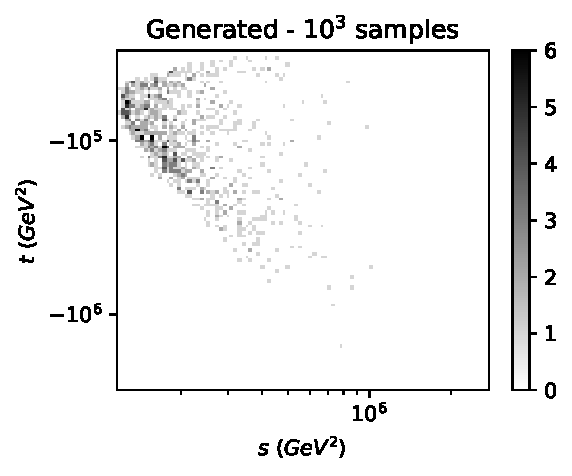
\includegraphics[width=0.32\textwidth]{plots/hardware/ibm_santiago/s-t_FAKE_IBM_1k.pdf}%
  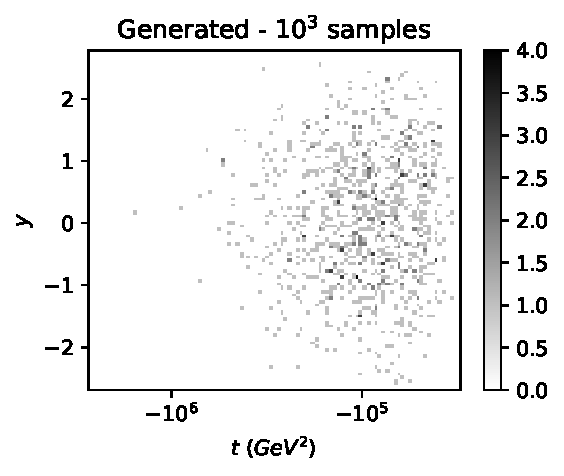
\includegraphics[width=0.32\textwidth]{plots/hardware/ibm_santiago/t-y_FAKE_IBM_1k.pdf}%
  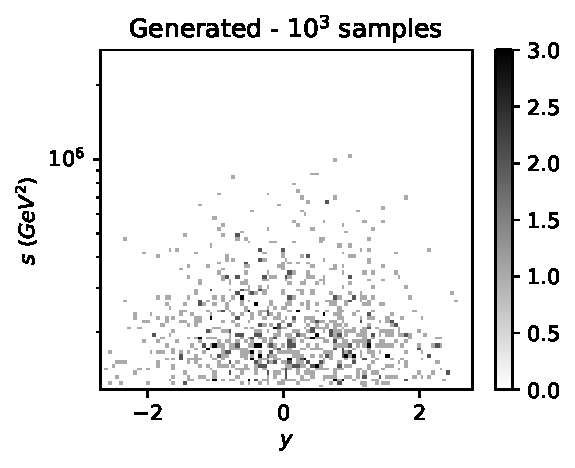
\includegraphics[width=0.32\textwidth]{plots/hardware/ibm_santiago/y-s_FAKE_IBM_1k.pdf}

  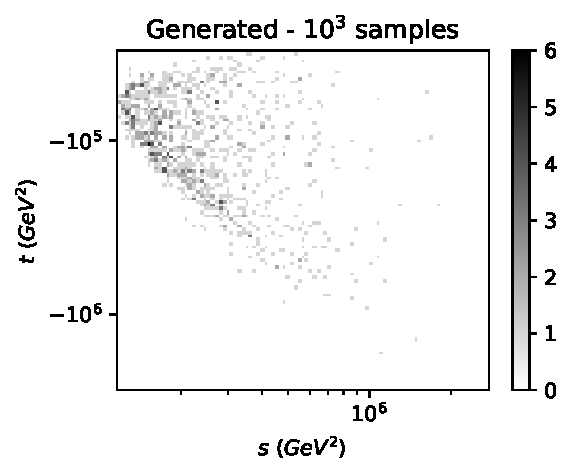
\includegraphics[width=0.32\textwidth]{plots/hardware/ionQ/s-t_FAKE_ionQ_1k.pdf}%
  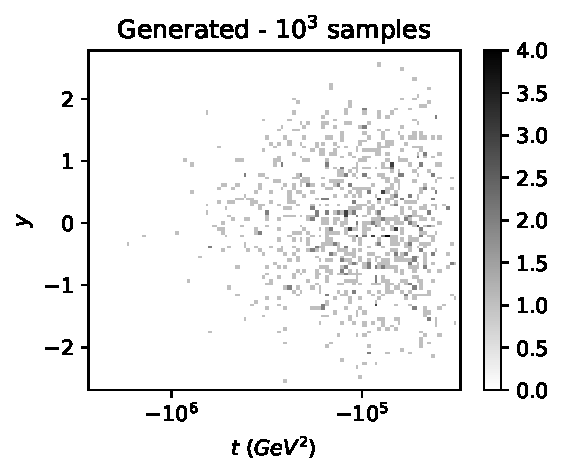
\includegraphics[width=0.32\textwidth]{plots/hardware/ionQ/t-y_FAKE_ionQ_1k.pdf}%
  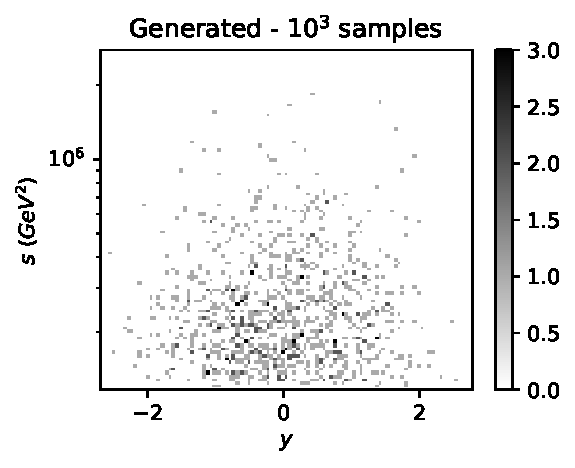
\includegraphics[width=0.32\textwidth]{plots/hardware/ionQ/y-s_FAKE_ionQ_1k.pdf}

  \caption{\label{fig:ionq}Example of two-dimensional sampling projections for
  $pp \rightarrow t\bar{t}$ production using the style-qGAN generator
  model on {\tt ibmq\_santiago} (top row) and IonQ (bottom row) trained with $10^4$ samples.}
\end{figure*}


\section{Conclusion}
\label{sec:conclusion}

In this work we proposed a novel quantum neural network model for the generation
of Monte Carlo events in the context of high energy physics (HEP). We have
investigated and identified the most suitable Ansatz for the parametrization of
a quantum generative network. Using quantum circuit simulation on classical
hardware, we show that qGAN generators are suitable for Monte Carlo event
simulation.

We highlight some advantages of the qGAN model when compared to the standard
machine learning methodology. From a hardware implementation point of view, the
possibility to write the specific qGAN circuit in a quantum processor, using its
primitives (gates), will accelerate the evaluations and training performance of
Monte Carlo sampling. We expect that real quantum devices will be more efficient
in terms of energy power than classical hardware based on hardware accelerators
such as graphical process units (GPUs).

Furthermore, we propose a reconstruction method for evaluating the qGAN model in
a real quantum device using measurements. This procedure brings all the
difficulties that are typical of experimental quantum hardware, including noise,
error corrections and decoherence. The implementation of accurate and stable
qGAN in a real quantum device still requires the development of hardware
architecture with lower gate error tolerances in comparison to the current
available machines.

On the other hand, our results should be considered as a proof-of-concept
exercise, given that the quantum simulation performance are still not
competitive with an equivalent machine learning implementation. The qGAN
approach may show advantages when more precise quantum devices will be
available.

Nevertheless, this is a first attempt to bridge the power of quantum machine
learning algorithms into the complexity of Monte Carlo simulation in HEP. We
wish that the approach presented here will inspire new HEP applications which
may benefit from quantum computing.

\section{Remaining to Do}
\commentDMG{Things still to do, from Oct. 6 meeting}
\begin{itemize}
\item Normalization sampling discussion/line
\item Maybe small discussion about Fig 3 to highlight why we include it -- typical GAN training convergence that shows that archicture does what it needs to do
\item Add Fig 5 discription of gray and white to make it clear (and so people know to look on computer if need be)
\item Keep working on this $10^4$ vs $10^5$ training versus generated vs reference
\item Green line for Fig 7 sanity check with different pull of $10^4$ reference samples. Anthony (+ Carlos for aid if need be)
\end{itemize}

\acknowledgments

C.B.-P. acknowledges Stavros Efthymiou for useful discussions about the
realization of the manuscript's code. S.C.~thanks Marco Zaro and Luigi Favaro for
discussions about classical GAN models applied to Monte Carlo events. This
project is supported by CERN's Quantum Technology Initiative. 
M.C.\ is supported by the European Union’s Horizon 2020 research and innovation programme under the Marie Skłodowska-Curie grant agreement number 843134.
SC is supported by the European Research
Council under the European Union's Horizon 2020 research and innovation
Programme (grant agreement number 740006). \commentJB{The authors acknowledge the support of the CloudBank EU as a pilot brockering cloud service at CERN, allowing
 for access to Amazon Web Services in order to run our algorithm on ionQ hardware.}


\appendix

\section{Noise simulation on IBM~Q device}
\label{sec:appendixnoise}

We have performed a noise simulation of our style-qGAN on IBM~Q device, taking as a device baseline the {\tt ibmq\_santiago}
5-qubit Falcon r4L quantum processor that we have used for our runs on actual IBM~Q hardware.

The noise model takes into account the readout error probability of each qubit (mean value of the probability
of reading $|1\rangle$ while being in state $|0\rangle$ and the probability of reading $|0\rangle$ while being in
state $|1\rangle$), the relaxation time constants of each qubit (relaxation time and dephasing time), the gate error probability
of each basis gate, and the gate length (timing of the gate) of each basis gate. The values are taken from the calibration information
of the selected device for the noise simulation. Note that this calibration is performed at regular intervals. The generation of our
$10^5$ samples on the actual machine has taken a week, meaning that the calibration parameters may have varied significantly
during the full run.

We show in Figure~\ref{fig:ibmnoise} the result of our noise simulation. In the middle row plots we compare our noise simulation
to the run on actual IBM~Q hardware, the latter being reported in Section~\ref{sec:deployment}. The plots show a significant amount
of white points, signalling that the noise simulation seems to capture most of the errors induced by running on an actual quantum
hardware and that errors beyond the parameters reported in the previous paragraph are subdominant. The KL distances displayed in
the lower row are also comparable to the KL distances reported in Figure~\ref{fig:ibm}. 

\begin{figure*}

  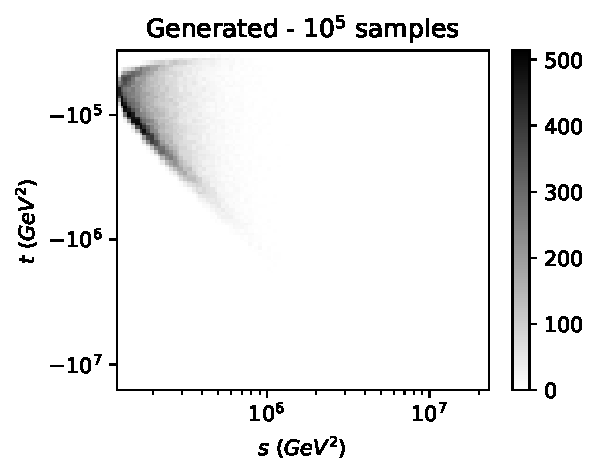
\includegraphics[width=0.32\textwidth]{plots/hardware_noise_simulation/s-t_FAKE_100k_noise-simu.pdf}%
  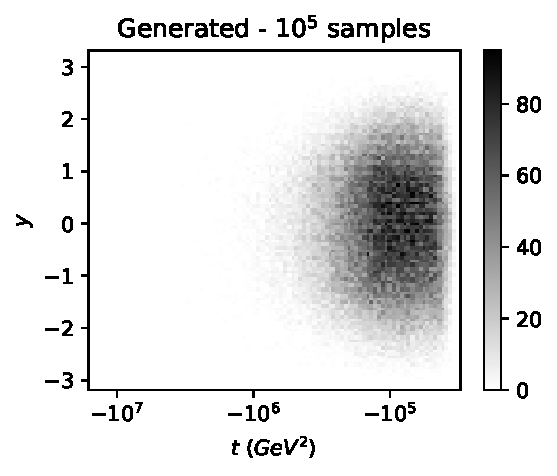
\includegraphics[width=0.305\textwidth]{plots/hardware_noise_simulation/t-y_FAKE_100k_noise-simu.pdf}%
  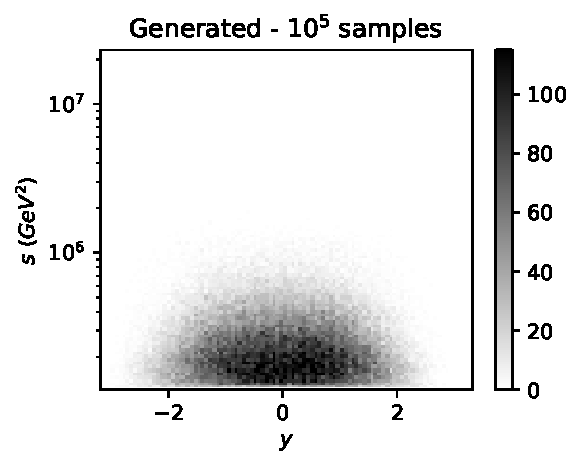
\includegraphics[width=0.31\textwidth]{plots/hardware_noise_simulation/y-s_FAKE_100k_noise-simu.pdf}

  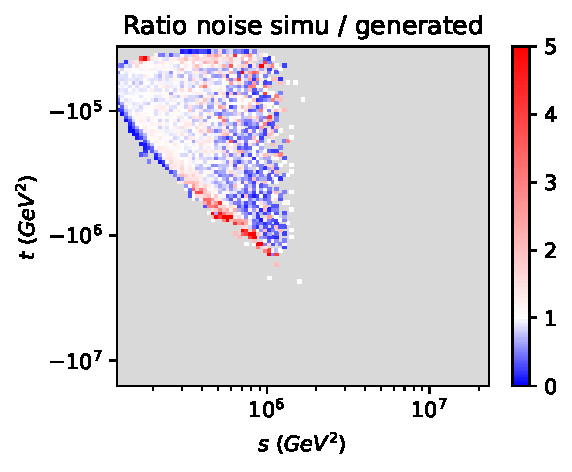
\includegraphics[width=0.32\textwidth]{plots/hardware_noise_simulation/s-t_RATIO_100k_noise-generated.pdf}%
  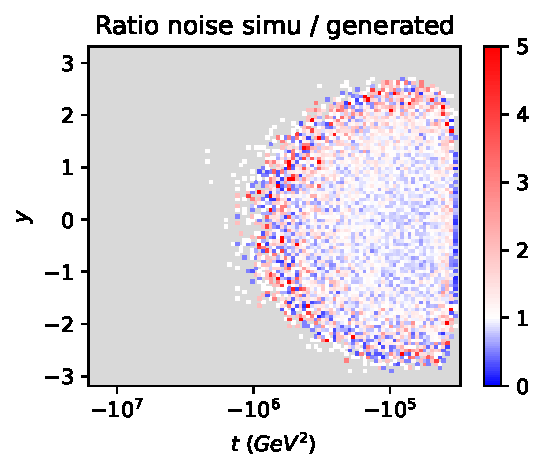
\includegraphics[width=0.305\textwidth]{plots/hardware_noise_simulation/t-y_RATIO_100k_noise-generated.pdf}%
  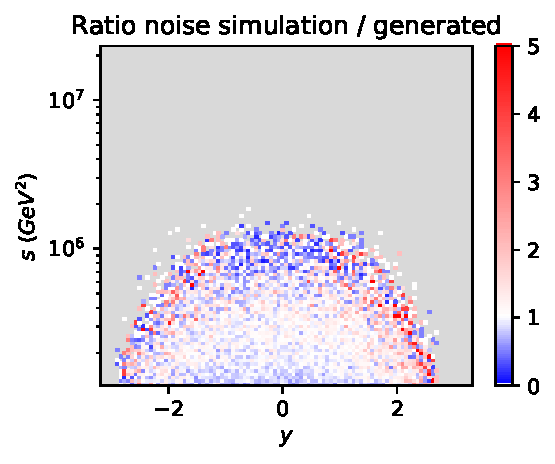
\includegraphics[width=0.31\textwidth]{plots/hardware_noise_simulation/y-s_RATIO_100k_noise-generated.pdf}

  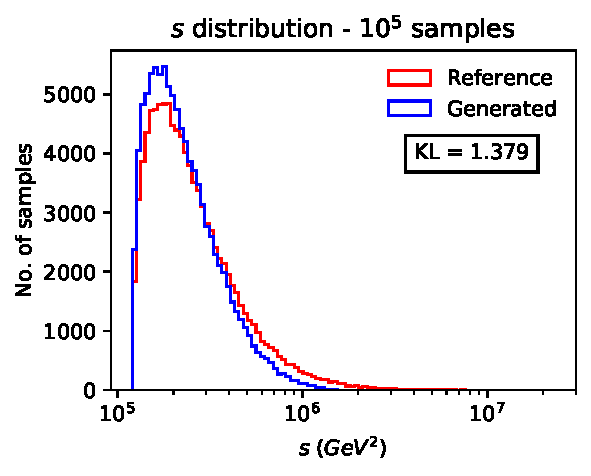
\includegraphics[width=0.29\textwidth]{plots/hardware_noise_simulation/s-distribution_LHCdata_100k_noise-simu.pdf}%
  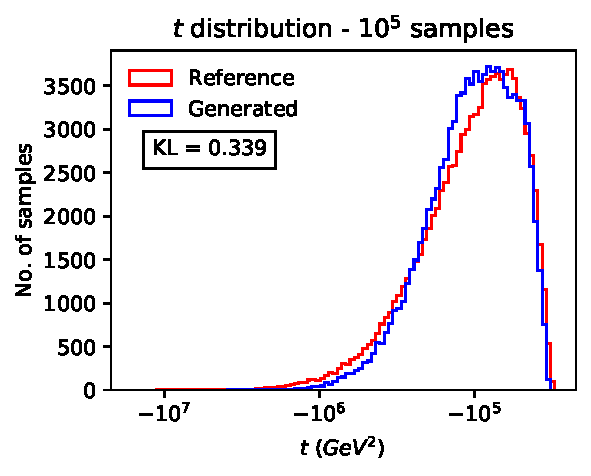
\includegraphics[width=0.29\textwidth]{plots/hardware_noise_simulation/t-distribution_LHCdata_100k_noise-simu.pdf}%
  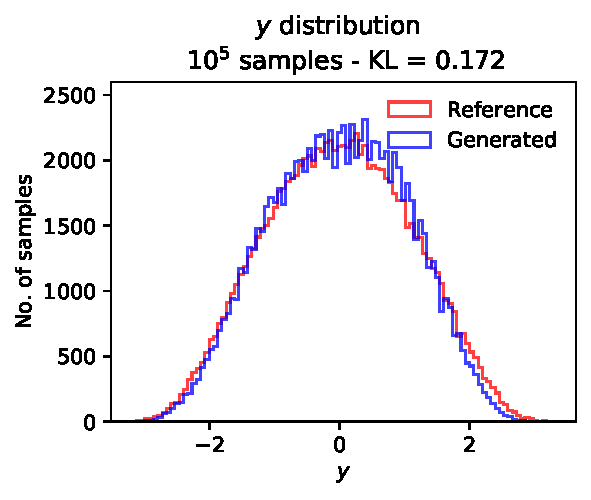
\includegraphics[width=0.29\textwidth]{plots/hardware_noise_simulation/y-distribution_LHCdata_100k_noise-simu.pdf}

  \caption{\label{fig:ibmnoise}Example of two-dimensional sampling projections for
  $pp \rightarrow t\bar{t}$ production using the style-qGAN generator
  model in a noise simulation of {\tt ibmq\_santiago} device (top row) trained
  with $10^4$ samples and the corresponding ratio to the generated samples on actual quantum hardware (middle row).
  Marginal samples distribution (bottom row) for each dimension compared to the the reference underlying prior MC
   distribution.}
\end{figure*}

We also compare our noise simulation to the noiseless simulation presented in Section~\ref{sec:lhc}.
The results shown in Figure~\ref{fig:ibmnoise2} indicate that while the noise has an impact, as expected, There are
still many points close the ratio 1, so that the style-qGAN still performs fairly well in a noisy environment. This has led us
to believe that running on an actual harware gives fairly good results.

\begin{figure*}

  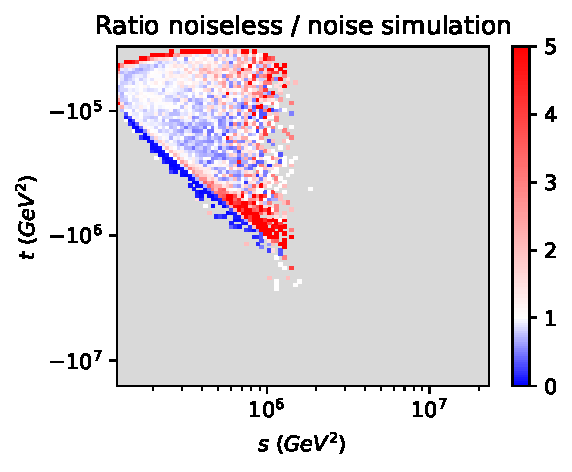
\includegraphics[width=0.32\textwidth]{plots/hardware_noise_simulation/s-t_RATIO_100k_noiseless-noise.pdf}%
  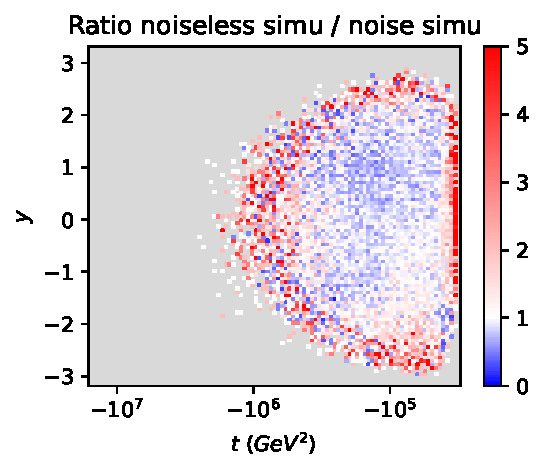
\includegraphics[width=0.305\textwidth]{plots/hardware_noise_simulation/t-y_RATIO_100k_noiseless-noise.pdf}%
  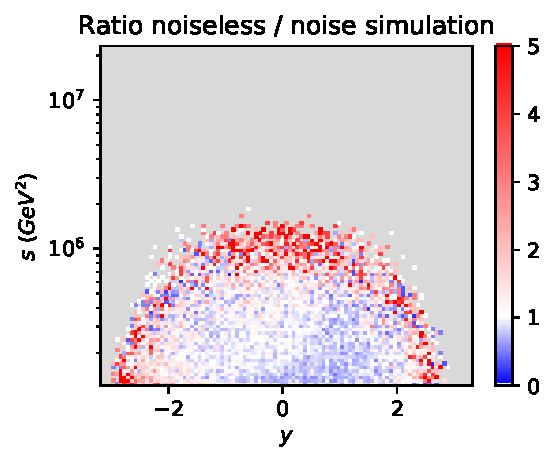
\includegraphics[width=0.31\textwidth]{plots/hardware_noise_simulation/y-s_RATIO_100k_noiseless-noise.pdf}

  \caption{\label{fig:ibmnoise2}Ratio of two-dimensional sampling projections using the noise simulation of {\tt ibmq\_santiago} device to the
    corresponding noiseless simulation presented in Section~\ref{sec:lhc}.}
\end{figure*}

\clearpage

\bibliography{qgan.bib}

\end{document}
